 \documentclass[12pt]{report}
%\documentclass[10pt]{article}
%\addtolength{\hoffset}{-3cm} \setlength{\topmargin}{-2.5cm} \setlength{\textheight}{25cm}
%\setlength{\footskip}{0.75cm} \setlength{\textwidth}{18cm} \setlength{\evensidemargin}{0.in}
%\linespread{0.9} \pagestyle{plain}



% \addtolength{\hoffset}{-0.35cm} \setlength{\topmargin}{-2cm} \setlength{\textheight}{24cm}
%\setlength{\footskip}{0.75cm} \setlength{\textwidth}{17.5cm} \setlength{\evensidemargin}{1.in}
% \documentclass[12pt,preprint]{aastex}
% \addtolength{\hoffset}{-0.5in}
% \setlength{\topmargin}{-0.75in}
% \setlength{\textheight}{9.4in}
%\setlength{\footskip}{0.75cm}
%\setlength{\textwidth}{16.75cm}
%\setlength{\evensidemargin}{1in}
%\setlength{\oddsidemargin}{0.5in}
%\linespread{1.0}
%\pagestyle{plain}
%\usepackage{graphics}
%\usepackage{color}
%\usepackage{times}
%\setcounter{section}{0}



\usepackage{datetime}
\usepackage{fancyhdr}
%\usepackage[outermarks]{titlesec}
\usepackage[utf8x]{inputenc}
\usepackage[T1]{fontenc}
\usepackage{amsmath}
\usepackage{amssymb}
\usepackage{epsfig}
\usepackage{graphics}
\usepackage{graphicx}
\usepackage[usenames]{color}
\usepackage{helvet}
\usepackage{times}
\usepackage{natbib}
\usepackage{import}
\usepackage{tabularx}
\usepackage{xspace}
\usepackage{scrextend}
%\usepackage{parskip}
\usepackage[normalem]{ulem}
\usepackage{scrwfile} % Stops "No room for a new \write" complaint
\usepackage{xcolor}
\usepackage{colortbl}
% Big tables summarizing plans:
\usepackage{pdflscape}
\usepackage{aas_macros}

\usepackage{afterpage}

\usepackage{pdftexcmds}

% Hyperref - always load as the last package!
\usepackage[linktocpage=false]{hyperref}
\hypersetup{
    colorlinks=true,
    citecolor=blue,
    filecolor=blue,
    linkcolor=blue,
    urlcolor=blue,
}

\usepackage{hypcap}

%\renewcommand{\thesection}{\Alph{section}}
%\setcounter{page}{1}
%\renewcommand{\thepage}{0-\arabic{page}}
\def\be{\begin{equation}}
\def\ee{\end{equation}}
\def\bea{\begin{eqnarray}}
\def\eea{\end{eqnarray}}
\def\bc{\begin{center}}
\def\ec{\end{center}}
\def\lg{\log_{10}}
\def\tcr{\textcolor{red}}
%\begin{document}


\linespread{1.1}
\addtolength{\hoffset}{-0.0cm}
\setlength{\topmargin}{-0.in}
\setlength{\textheight}{8.25in}
\setlength{\footskip}{1.5cm} %{0.75cm}
\setlength{\textwidth}{6.25in}
\setlength{\evensidemargin}{1in}
\setlength{\oddsidemargin}{0in}

\setlength\parindent{0pt}
\setlength{\parskip}{0.3cm}
%  \usepackage{paralist}
%\setlength{\pltopsep}{0pt}
%\setlength{\plpartopsep}{0pt}

\def\tcr{\textcolor{red}}
\def\tcb{\textcolor{blue}}
\def\accent{\it}
\def\vs{\vspace{0.5cm}}
\def\hs{\hspace{0.5cm}}
\urlstyle{rm}

%--------------------------------------------------------------
%--------------------------------------------------------------

\begin{document}

\pagestyle{fancy}
\fancyfoot{}% clear all footer fields
\fancyfoot[R]{\thepage}  % page number in "outer" position of footer line

\fancyhead[L]{ \rm Facilitating Cosmology Measurements from LSST}
\fancyhead[R]{}
\renewcommand{\footrulewidth}{1pt}

%{\bf General guidelines for April 18th: we should produce brief "white papers" describing the science in greater detail and
%		quantifying the capabilities needed. Similar to a rough draft of an NOAO observing proposal.
%		It has the same elements of compelling science, technical description and quantitative
%		statement of resource needs. But does not have to be very polished.}

\begin{centering}
{\huge{\bf{{Facilitating Cosmology Measurements from LSST}}}}


{\it{\bf Executive Summary:}}
\end{centering}
%
%{\it One paragraph summarizing (1) the main science goals, (2) needed capabilities (top level detailed specifications such as resolution, wavelength coverage, FOV, multiplex), (3) estimate of demand to meet science goals (e.g., number of nights, fiber hours), and (4) priorities for each capability (3-tier: critical, very important, important). The chapter should be $\sim$10 pages. }

Almost all LSST studies of cosmology can be enhanced by the addition of spectroscopic information.  Some of the most critical needs, as they affect essentially all cosmological probes, are training of photometric redshifts (i.e., obtaining spectroscopic samples to refine photo-z algorithms) and photo-z calibration (i.e., characterizing the actual biases and errors of photo-z algorithms).  The former will require an investment of $\sim$ a year or more of observing time on a wide-field ($>20$ arcmin, with $>1$ degree preferred), highly-multiplexed ($>2000\times$), medium-resolution ($R>4000$ in the red), broad-wavelength coverage (0.4--1.0$\mu$m minimum, 0.3--1.5$\mu$m preferred) multi-object spectrograph on an 8m-class telescope.  Calibration of photometric redshifts via cross-correlation techniques will require overlap of a DESI-like galaxy and quasar survey with the LSST footprint.  A number of cosmological probes can utilize such a spectrograph or, in some cases, existing or planned spectrographs on large telescopes with smaller fields of view but otherwise similar capabilities to mitigate potential systematics or provide new constraints on modified gravity theories.

For efforts to constrain cosmology using strong gravitational lensing, adaptive optics imaging and IFU spectroscopy on 8-30m telescopes will be most critical.  Instrumental requirements include a resolution of $\sim 0.1$ arcsec FWHM, field of view of 4 arcsec diameter, and (for spectroscopy) $R \sim 4000 - 5000$ over a wavelength range of 1.0-2.2$\mu$m.   Total time requirements are roughly 30 hours for imaging and 100 hours for spectroscopy to cover a sample of 100 particularly high-quality strong lens systems.  

Supernova cosmology will require spectroscopy of thousands of active supernovae to investigate supernova physics and constrain the properties of supernovae which are not associated with a visible host galaxy.  Additionally, spectroscopic redshift measurements for hosts of supernovae whose spectra were not obtained when they were active can greatly enhance the size of the samples used for constraining cosmology.  Direct supernova spectroscopy will require broad wavelength coverage (0.3--1.0$\mu$m minimum, $\sim$ 0.3 -- 2.5~$\mu$m preferred), modest resolution ($R>\sim 100$), high efficiency single-object spectrographs on 4m, 8-10m, and GSMT telescopes, with total time requirements over the life of LSST of 300-900 telescope-nights.  Supernova host spectroscopy is most efficiently conducted with very large field, highly-multiplexed spectrographs similar to those required for photometric redshift training and calibration; redshifts can be obtained for the majority of supernovae in deep drilling fields with $\sim 15-30$ nights of observations per year on a DESI-like spectrograph on a 4m telescope.    

\section{Introduction}

A key driver for LSST is to investigate the nature of the source of the accelerating expansion of the Universe.  The primary possibilities are that there is a new, unknown component which dominates the energy density in the Universe today (commonly labeled ``dark energy''), or else that Einstein's theory of General Relativity (GR) fails to provide an accurate description of the action of gravity on large scales (a class of models generally referred to as ``modified gravity'' theories).  Many of the planned cosmological measurements from LSST can also be used constrain neutrino masses and dark matter properties.  {\bf By strengthening LSST cosmological constraints and mitigating potential systematics, the work described in this chapter will help LSST to address a key objective identified in the {\it New Worlds, New Horizons} report, studying the Physics of the Universe.}

The constraining power of almost all LSST probes of cosmology (as well as other extragalactic work with LSST) will be greatly strengthened by the addition of spectroscopic redshift measurements for training photometric redshift algorithms.  Obtaining such samples requires spectrographs that maximize multiplexing, areal coverage, wavelength range, resolution, and telescope aperture, as described below.  Studies of cosmology using strong gravitational lensing also requires adaptive optics IFU observations of the highest-priority lens systems in order to obtain precision source precisions and tighten constraints; instruments currently available on 8-10m telescopes or planned for ELTs are well-suited for this work.


%%Almost all LSST probes of cosmology will be greatly strengthened by the addition of spectroscopic redshift measurements for large samples of galaxies.  
%Spectroscopic samples to train photometric redshift algorithms will improve constraints from almost all LSST extragalactic studies, including cosmology.
%%;. spectroscopy obtained with the same instruments can be important for investigating the effects of intrinsic alignments between galaxies on the observed weak lensing signal or for improving the use of galaxy clusters as a cosmological probe, amongst other applications.  
%This work will benefit from spectrographs that maximize multiplexing, areal coverage, wavelength range, resolution, and telescope aperture, as described below.  {\bf By strengthening LSST cosmological constraints and mitigating potential systematics, this spectroscopy will help LSST to address a key objective identified in the {\it New Worlds, New Horizons} report, studying the Physics of the Universe.}
%
%Larger, wider-area samples of bright galaxies and QSOs with redshifts, such as those provided by DESI, can be used to accurately calibrate the results of photometric redshift algorithms via cross-correlation measurements; the same samples can contribute to cross-correlation studies of intrinsic alignments and LSST large-scale structure.  We will focus on the training and calibration of photometric redshift algorithms in this section; however, a broad swath of dark energy science would benefit from the same capabilities, and we highlight a few examples at the end of the section.
%


\section{Science Case 1: Multi-Object Spectroscopy for Training and Calibrating Photometric Redshifts}

%A) Photo-z training and calibration (including in cluster regime, spectroscopy of blends identified in space-based imaging)
%		- JN, AvdL, WD, SS, MD
\label{sec:photoz}

{\it Jeffrey Newman, Will Dawson, Elise Jennings, Anja von der Linden, Rachel Mandelbaum, and Samuel Schmidt }

LSST dark energy constraints, as well as almost all LSST extragalactic science, will be critically dependent upon photometric redshifts (a.k.a. photo-$z$'s): i.e., estimates of the redshifts of objects based only on flux information obtained through broad filters.  In this section, we describe the utilitization of spectroscopy for photometric redshifts for two separate purposes:
\begin{itemize}
\item {\it Training}, that is, making algorithms more effective at predicting the actual redshifts of galaxies, reducing random errors.  Essentially, {\bf the goal of training is to minimize all moments of the distribution of differences between photometric redshift and true redshift}, rendering the correspondence as tight as possible, and hence maximizing the three-dimensional information in a sample; and
\item {\it Calibration}, the determination of the actual bias and scatter in redshifts produced by a given algorithm (for most purposes, this reduces to the problem of determining the actual redshift distribution for samples selected based on some set of properties).  Essentially, {\bf the goal of calibration is to determine with high accuracy the moments of the distribution of true redshifts of the samples used for a given study}.
\end{itemize}
Different datasets will be needed for each of these purposes.  However, as will be described below, the same instrumental capabilities -- and often the same datasets -- needed for photometric redshift training or calibration can also contribute to LSST cosmology in a variety of other ways; we will describe some of these applications at the end of this section.






\subsection{Science Goals}
%
% {\it Describe your science goals here, as in the scientific justification of an NOAO proposal. If you have multiple science goals, you can either describe them all here, or replicate the science, technical, and capabilities sections for each goal. Just create one summary table for the entire program.  }

%NOAO guidelines:
%
%The scientific justification should explain the overall goals of
%your program in the context of your field, as well as the importance
%of your program to astronomy.
%Writing a good scientific justification is an art.  It takes
%skill and practice.  And it requires a good scientific idea.
%This last you must supply but a few general guidelines
%about proposal writing might still be helpful...
%
%\begin{itemize}
%\item
%State succinctly and clearly the problem you are trying to solve
%and the progress that will be made toward doing so if the proposed
%observations are successful.  If the review panel members have to work hard
%even to understand what you want to do, they are unlikely to be
%sympathetic to your proposal.
%
%\item
%Explain clearly why the project is important and how it
%relates to the broad context and important issues in your field.
%Many proposals focus too tightly on a specific observational
%goal (e.g. ``measure the velocity dispersion of this cluster of galaxies'')
%without explaining why it is important or how it relates to a
%significant question about the Universe.
%
%\item
%Be specific.  If your observations will ``constrain theoretical
%models,'' then discuss what will be constrained and why those
%constraints matter.  Make sure the review panel understands exactly why
%the observations you propose will make a difference in your field,
%and exactly how the observations will refine or
%require changes in the theory.
%
%\item
%Keep it simple.  Try to focus on the central idea of your proposal.
%Complex arguments are hard to explain and hard for the panel members to follow.
%Distracting tangential arguments obscure the theme of your proposal.
%
%\item
%Include a figure to help explain what you want to do.  Sample
%data or model predictions shown in a figure often help clarify
%complex arguments for the panel members.
%
%\item
%Keep it short.  Never exceed a page for the text of the scientific
%justification, and never reduce the font size.  It may even help to
%be a little under a page, and increase the font size a little!
%Organize your presentation with paragraphs, headings, and bullets
%so it is easy to read.

\label{sec:photoz_just}

%LSST dark energy constraints, as well as almost all LSST extragalactic science, will be critically dependent upon photometric redshifts (a.k.a. photo-$z$'s): i.e., estimates of the redshifts of objects based only on flux information obtained through broad filters.
%
%Improvements that yield higher-quality, lower-RMS-error photo-$z$'s will result in smaller random errors on parameters of interest and enable analyses in narrower redshift bins; while systematic errors in photometric redshift estimates, if not constrained, may dominate all other uncertainties when studying cosmological parameters.  Both optimizing and calibrating photo-$z$'s are dependent upon obtaining secure redshift measurements from spectroscopy.

%\subsection{\Training}

{\bf Training:} Photo-$z$ methods generally use samples of objects with known $z$ to develop or
refine algorithms, and hence to reduce the random errors on individual photometric redshift
estimates. This will result in smaller errors on cosmological parameters of interest and
will enable analyses in narrower redshift bins.  Larger and more complete training sets result in smaller
RMS errors in photo-$z$ estimates, increasing LSST's constraining power.
% For instance, LSST delivers photo-$z$'s with an RMS error of $\sigma_z \sim 0.025(1+z)$ for $i<25.3$ galaxies in simulations with perfect template knowledge and realistic photometric errors, whereas photo-$z$'s in actual samples of similar S/N have delivered $\sigma_z \sim 0.05(1+z)$.
With a perfect training set of galaxy redshifts down to LSST magnitude limits, we could achieve the system-limited performance; this would improve the Dark Energy Task Force figure of merit from LSST lensing+BAO studies by $\sim25$\%, with greater impact in other areas (e.g., studies of galaxy clusters).  {\bf Better photometric redshift training will improve almost all LSST extragalactic science, and hence addresses a wide variety of decadal science goals.}  To enable this, we need secure spectroscopic redshifts for as wide a range of galaxies as possible down to the $i=25.3$ magnitude limit of the LSST weak lensing ``gold sample'').

%\subsection{Calibration}

{\bf Calibration:} Similarly, secure spectroscopic redshifts are needed for {\em calibration}, i.e., the
empirical determination of photo-$z$ bias and scatter.  {\bf Inadequate calibration will lead to
  systematic errors in almost all extragalactic science cases with LSST and hence many decadal science priorities}.
% It is estimated that the true mean redshift for each sample used for LSST cosmology (e.g., objects selected to be within some bin in photometric redshift) must be known to $\sim 2\times10^{-3}(1+z)$, i.e., 0.2\%.
Extremely high completeness (>99.9\%) in the spectroscopic samples used for training would enable
LSST calibration requirements to be met directly. However, existing deep redshift samples lack secure redshifts for a systematic 20\%-60\% of their targets; it is therefore quite likely that future deep redshift samples will not solve the calibration problem.

Instead, we can use cross-correlation methods to calibrate photo-$z$'s.  These techniques correlate
the positions on the sky of objects with known $z$ with the positions of the galaxies whose redshift
distribution we aim to characterize.  We can then exploit the fact that bright galaxies trace the
same underlying dark matter distribution as fainter objects, enabling the determination of the $z$
distribution for purely photometric samples with high accuracy.  Photo-$z$ calibration via
cross-correlations requires redshifts for very large numbers of objects over a wide area of spatially overlapping sky,
spanning the full redshift range of LSST targets of interest.




\subsection{Technical Description }

% {\it Give a technical description of your program, describing e.g., sample size and properties, justification of spectral or spatial resolution, wavelength, target density, etc.}

%NOAO guidelines:
%The review panel looks to this section to find out about the overall
%strategy of your observational program.  Why do you need the telescopes
%and instruments you request? How are your targets selected?
%Why do you need spectroscopy or imaging, and what measurements will
%you make from the data?  Why is your approach to be preferred over
%some other approach, what must the minimum sample size be to achieve
%your scientific goals (and why), and why are your
%observations likely to be better than previous work in the field?

\label{sec:photoz_design}

{\bf Training:} A previous whitepaper on {\it Spectroscopic Needs for Imaging Dark Energy Experiments} \citep{Newman15} has explored in detail the minimum characteristics a photometric redshift training set should have.  We summarize those conclusions here.  In short, we require:

\begin{itemize}
\item {\bf Spectroscopy of at least 30,000 objects down to the survey magnitude limits}, in order to characterize both the core of the photo-$z$/spectroscopic-z relationship and outliers (cf. \citealt{MaHuterer}, \citealt{BernsteinHuterer}, and \citealt{Hearin10}); this will require large exposure times on large telescopes.
\item {\bf High multiplexing}, as obtaining large numbers of spectra down to faint magnitudes will be infeasible otherwise.
\item {\bf Coverage of as broad a wavelength range as possible}, in order to cover multiple spectral features, which is necessary for getting the required {\bf highly-secure} redshifts.  At minimum, spectra should cover from $\sim 4000$ to $\sim 10,000$ Angstroms, but coverage from $\sim 0.3$ to $\sim 1.5\mu$m would be advantageous.
\item {\bf Moderately high resolution ($R>\sim 4000$) at the red end}, critical as it enables secure redshifts to be obtained from the [OII] 3727 Angstrom doublet alone.  High resolution also enables sensitive spectroscopy over the $\sim 90\%$ of the spectrum that lies between the skylines (cf. Newman et al. 2013).
\item {\bf Field diameters $>\sim20$ arcmin}, needed to span multiple correlation lengths to enable accurate clustering measurements.
%This is key for enabling the training samples to be well-understood, providing synergistic galaxy evolution science, and enabling the spectra obtained to be utilized with cross-correlation techniques; it also reduces sample/cosmic variance in the training set.  A typical correlation length of $r_0 \sim 5 h^{-1}$ Mpc comoving corresponds to $\sim 7.5$ arcmin at z=1 and 13 arcmin at z=0.5; hence,
Larger ($>1$ deg) fields would be even better, particularly at low redshifts.
\item And finally, {\bf coverage of as many fields as possible ($\sim 15$ minimum)}, in order to minimize the impact of sample/cosmic variance.
%Cunha et al. (2012) estimated that 40-150 $\sim$ 0.1 deg$^2$ fields would be needed for DES for sample variance not to impact errors; however, we can do somewhat better by taking advantage of the fact that the variance itself is directly observable via the field-to-field variation in redshift distributions.  Nevertheless,
%with fewer than $\sim 15$ independent (i.e., widely separated) fields, it would be difficult to measure dispersions in counts amongst the fields directly, as measurements of standard deviations are broad and highly skewed for small N. We thus require at least this many fields.
\end{itemize}


{\bf Calibration:} As described in \citet{Newman15},  cross-correlation calibration of photometric redshifts for LSST should require spectroscopy of a minimum of $\sim 5 \times 10^4$ objects over multiple independent $>100$ square degree fields, with coverage of the full redshift range of those objects whose photometric redshifts will be calibrated (for LSST dark energy science, this is essentially $0<z<3$).



\subsection{Needed Capabilities and Estimate of Demand}

% {\it Describe the needed capabilities and demand (e.g., estimate of observing time) that flow down from the science and technical considerations. If applicable, describe the time critical nature of the required capabilities (do you need to have the capabilities while LSST is carrying out the survey or can you do the follow up later?) }

{\bf Training:} In principle, a number of spectrographs currently in existence or being planned have sufficient wavelength coverage and spectral resolution to obtain secure redshifts over a wide range of galaxy properties for photo-$z$ training.  However, the time required will depend on the instrumental and telescope characteristics.  If sky coverage is low, the limiting factor will be how many tilings of the sky will be needed to cover $>15$ fields that are 20 arcmin in diameter.  If multiplexing is low, the limiting factor will be how many tilings are needed to reach 30,000 spectra.  Finally, if both of these factors are high enough that each field need only be observed once, the limiting factor will be how much exposure time it takes the telescope to achieve the desired depth.  Formulae for how exposure time scales in these scenarios are given in \citet{Newman15}.
%
%The actual time required for a survey in each of these scenarios will be:
%
%{\it FOV-limited}:  $t_{observe}$ =(280 nights) $\times$ ($N_{fields}$ / 15) $\times$ (314 arcmin$^2$ / area per pointing )$\times$( Equivalent Keck/DEIMOS exposure time / 100 hours) $\times$ (0.67 / observing efficiency) $\times$ (76 m$^2$  / telescope effective collecting area) $\times$ (0.3 / [telescope + instrument throughput]),
%
%{\it Multiplex-limited}:  $t_{observe}$ =(280 nights) $\times$ ($N_{objects}$ / 3$\times10^4$) $\times$ (2000 / Number of simultaneous spectra)$\times$(Equivalent Keck/DEIMOS exposure time / 100 hours) $\times$ (0.67 / observing efficiency) $\times$ (76 m$^2$  / telescope effective collecting area) $\times$ (0.3 / [telescope + instrument throughput]), or
%
%{\it Fields-limited}:  $t_{observe}$ =(280 nights) $\times$ ($N_{fields}$ / 15) $\times$ (Equivalent Keck/DEIMOS exposure time / 100 hours) $\times$ (0.67 / observing efficiency) $\times$ (76 m$^2$  / telescope effective collecting area) $\times$ (0.3 / [telescope + instrument throughput]),
%
%where $t_{observe}$ is the total clock time required for observations (including overheads and weather, which both reduce observing efficiency); $N_{fields}$ is the total number of fields to be observed; and $N_{objects}$ is the total number of objects to be observed.
%For any given telescope/instrument combination, the actual exposure time required will be the greatest out of the fields-limited, FOV-limited, and multiplex-limited values.
100 hours' Keck/DEIMOS exposure time would be sufficient to achieve the same signal-to-noise for $i=25.3$ objects that DEEP2 obtains at $i \sim 22.5$; at that magnitude, DEEP2 obtained secure redshifts for $\sim 75\%$ of targets.  A spectrograph with broader wavelength range or higher spectral resolution would be expected to do at least as well as this at equivalent signal-to-noise.

\citet{Newman15} tabulates the properties of a variety of current and upcoming spectrographs and estimates the total time they would require to complete the proposed survey.  It would take more than 10 years with Keck/DEIMOS, 5 years with Mayall/DESI,  $\sim1.8$ years with TMT/WFOS, just over 1 year with Subaru/PFS, or as little as 4-5 months on GMT or E-ELT (depending on the final characteristics of instruments whose design is still in flux).  If less telescope time is available, it will be necessary to either allow spectroscopic redshift failure rates to increase or to reduce the depth of the sample; it is likely that the former would have smaller impact on photometric redshift training.  By design, this training sample would also be sufficient to meet LSST calibration requirements {\bf if} spectroscopic redshift failure rates of order $\sim 0.1\%$ could be achieved.  However, based on past experience (with 20-60\% failure rates) we expect to need less direct methods for calibrating photometric redshifts.

We note that the results of this survey -- a set of galaxies spanning the full range of galaxy properties down to the LSST magnitude limit with a maximal amount of spectroscopic information -- will enable a wide variety of galaxy evolution science going well beyond just the training of photometric redshifts.  A number of applications for such a sample are discussed in Chapter XYZ; the sample described in that chapter has considerable overlap, but (if IR spectral coverage is available) somewhat shorter estimated exposure times.  Ideally, this spectroscopy would occur early in the lifetime of LSST, but training redshifts will be useful whenever they are obtained.

{\bf Calibration:} LSST photometric redshift calibration requirements should be met by the overlap between LSST and planned baryon acoustic oscillation experiments.
%Those projects are optimized by targeting the brightest galaxies at a given redshift over the broadest redshift range and total sky area possible; this matches the needs for cross-correlation measurements well.  For photometric redshift calibration, all redshifts used must be highly secure ($>$99\% probability of being correct); however, here incompleteness is not an issue.
For instance, DESI should obtain redshifts of $>\sim$30 million galaxies and QSOs over the redshift range $0 < z < 4$ over more than 14,000 square degrees of sky \citep{DESI}.  It is expected to have $>4000$ square degrees of overlap with LSST.
%Absorption-line systems detected in DESI QSO spectra can provide even more redshifts at low z (Menard et al. 2013).
%We anticipate that DESI will provide several million redshifts within the footprint of LSST.
%As can be seen in Figure XYZ, DESI will allow detailed analyses of photometric redshift calibration, providing multiple cross-checks for systematics.

However, the DESI survey will cover only the northern portion of the LSST sky.  Photometric redshift performance may not be the same there as elsewhere in the LSST footprint (e.g., due to airmass differences), which could yield a miscalibration when applied to LSST as a whole.  This risk can be mitigated by DESI-like spectroscopy in the south.  There are plans to conduct a DESI-like survey with the 4MOST instrument that would fulfill this need well.  If this does not happen, it would be extremely valuable to have access to a DESI-like spectrograph (with wide field of view, $\sim 5000\times$ multiplexing, full optical coverage, sufficient resolution to split [OII], and a $\sim 4m$ diameter telescope aperture) in the Southern hemisphere.  With such an instrument, covering the non-DESI LSST footprint would take comparable observing time to the original DESI survey.

\subsection{Other applications of the required instrumentation}

The same instrumentation needed for a photometric redshift training survey would be well-suited to address a number of other important issues  affecting cosmological measurements with LSST.  We describe a key example here.

{\bf Intrinsic Alignment Studies:} Some of the strongest LSST constraints on dark energy are
expected to come from measurements of the apparent shearing of galaxy images by weak gravitational
lensing.  Characterizing and mitigating systematic uncertainties will be critical to ensure that
LSST weak lensing measurements are not systematics dominated.  The photometric redshift training and
calibration datasets will address one important systematic for weak lensing, but the multi-object
spectroscopy can also help characterize and constrain another systematic: intrinsic alignments (IA)
of galaxy shapes with the cosmic web, which are a contaminant to weak lensing measurements \citep{2015SSRv..193....1J}.

%Several
%methods have been developed for mitigating this systematic, including nulling, forward modeling, and self-calibration.
Existing methods of mitigating this systematic all have limitations, making it important also to
explore intrinsic alignment effects directly, using redshifts to determine
which galaxies are in physical proximity to each other.
%This direct exploration will provide
%intrinsic alignments models as inputs to the mitigation methods that need models.  % JAN: I added that last sentence in response to a question from Joan Najita:
%How critical is the spectroscopy? The first paragraph mentions several methods -- do they all need spectroscopy? If not, how much does the spectroscopy add to the science result? (Is it "nice to have" or "critical"?)
%In particular, we are lacking knowledge of how intrinsic alignments scale with
%galaxy type, luminosity, and redshift at $z> 0.5$.
%However, we need similar information both for
%galaxies at higher redshifts and for blue galaxies in general in order to develop reasonable priors for carrying out the WL analysis with LSST. Generally, this
%requires both good imaging and redshift information, in order to both localize the galaxy pairs in
%3D and measure galaxy shapes.   LSST data itself will ultimately be quite informative about
%IA despite the size of the photo-$z$ errors, but there is still value in
%Large sets of spectroscopic redshifts can provide strong external priors on
%IA models.
% using spectroscopic redshifts, because IA are degenerate with other systematics (photo-$z$ errors and certain shear systematics).
%In principle, a
A direct measurement of IA would require a spectroscopic or spectro-photometric dataset that covers substantial
contiguous areas ($\gtrsim$1 deg$^2$) while sampling a
{\em representative} galaxy sample of tens of thousands of galaxies at minimum.
%As an example of the required field sizes, 1 degree at $z=0.8$ corresponds to a distance of $\sim 35 h^{-1}$ Mpc comoving, which should be well-suited to
%constraining IA models on the $\lesssim 10 h^{-1}$Mpc scales where existing theoretical models are
%most uncertain.  The desirability of large field sizes is somewhat in tension with the approach of surveying many modest-size fields to mitigate sample/cosmic variance as employed in the ``training'' dataset described in
%Sec.~\ref{sec:design}), but l
Larger-field spectrographs such as Subaru/PFS could provide the necessary areal coverage and sampling as part of a photo-$z$ training survey.  If the photo-$z$ training survey covers smaller fields, supplemental spectroscopy with the same sort of instrument required for training work could be necessary.
%it is quite possible that a training set that is still well-suited for IA studies could be developed (we note, for instance, that if the Subaru/PFS spectrograph were used for the training samples, it would have a minimum field size well-suited for IA studies).

Because high redshift precision is not needed, an alternative approach would be to supplement LSST photo-$z$'s with many-band narrow-band imaging or low-resolution spectroscopy; however, high signal-to-noise at faint magnitudes would be necessary, requiring new instrumentation on large telescopes.
%
%An alternative a
%It is worth noting that, although the medium-resolution MOS spectroscopy envisioned for photo-$z$ training could serve the needs of IA characterization, the redshift RMS accuracy needed for this purpose is not particularly high.  Many-band narrow-band imaging, low-resolution spectroscopy, or spectro-photometric redshifts similar to those from the PRIMUS survey could deliver sufficiently low errors, presuming that highly-secure redshifts are obtained from them (the $\sim 5--10\%$ incorrect-z rates from PRIMUS would likely be problematic here). However, the galaxies for which redshifts to characterize IA for LSST are required are much fainter than those studied in previous low-resolution surveys; new instrumentation on larger telescopes would be needed to meet this goal.
Another alternative would be to constrain IA using cross-correlations with spectroscopic galaxies instead of employing
autocorrelation measurements (cf. \citealt{Blazek} and \citealt{Chisari}), which could utilize the same data needed for the photo-$z$ cross-correlation calibration method.
%More exploration is needed to determine precise survey design requirements for this supporting science case, but we anticipate they will be
Having both photo-$z$ training and calibration sets available, and making sure they are
well-optimized for IA purposes, will provide us with multiple potential routes to developing and
testing IA models, maximizing the chances of success.


\subsection{Applications requiring smaller fields of view}

Although the most urgent cosmological needs for multi-object spectroscopy require wide fields of
view (of order 0.5 -- 1 degree) to span the typical scales of large-scale structure, certain science
cases require a dense placement of spectra in smaller $\sim 5-10$ arcmin fields of view (though other requirements are similar to those for wide-field spectroscopy).  Because the relevant galaxies are relatively tightly packed on the sky and multiplex requirements are not high, existing or planned slit spectrographs such as Keck/LRIS, Keck/DEIMOS, Gemini/GMOS, and TMT/WFOS may be suitable.  If fibers can be packed tightly enough, a wide-field multiobject spectrograph could also contribute to these activities, but may be less optimal.  We discuss a few example applications of such spectroscopy below. 

{\bf Galaxy Cluster Studies:}
Cosmology with the cluster mass function may become one of the most powerful probes of the cosmology in the LSST era, if cluster masses can be measured to high enough accuracy and precision (Cosmic Visions report; Krause and Eifler 2016).  Moreover, they provide avenues for probing gravity as well as the properties of dark matter.  Multi-object spectroscopy plays a major role on all of these:

\begin{itemize}
\item Photo-z uncertainties specific to cluster fields present one of the primary systematics in cluster weak-lensing analyses to anchor the absolute cluster mass calibration (Applegate et al. 2014, DESC white paper).  Galaxies along a line of sight that contains a cluster are more likely to be at the cluster redshift than would be expected based upon posterior probability distributions calculated without any reference to position.  Such modulation of the prior should depend upon both cluster redshift and mass.  Some amount of training datasets (targeting galaxies selected by their photo-z's to be behind clusters) is necessary for this work to identify (possibly unexpected) failure modes of mistaking cluster galaxies for background galaxies. FOVs of $\gtrsim 20$~arcmin are ideal for targeting cluster fields at $z_{\rm Cl}\gtrsim0.2$.  Constraints on the wavelength coverage are somewhat reduced for investigating only the cluster redshift failure mode. Accordingly, existing instruments (e.g. DEIMOS) are already well-suited for this work, especially if the large-scale photo-z training surveys are predominantly performed with larger-area, sparser spectrographs.  Training sets should target clusters over a range of redshift, acquiring ~500 background redshifts per cluster to fully characterize the accuracy of $p(z)$ distributions in cluster fields.  In addition, cross-calibration datasets can be a sensitive test for residual cluster galaxy contamination. These are easier to obtain, targeting (bright) red-sequence galaxies.  Spectroscopy of $\sim 100--300$ galaxies in each of $\sim 20--50$ clusters would be useful for this purpose.  
\item The combination of weak lensing with dynamical mass probes (e.g., measurements of galaxy velocities within clusters) can be used to test non-GR theories of gravity, which could provide an alternative explanation for the cosmic acceleration commonly described to dark energy. The same spectroscopy used to characterize photometric redshifts around clusters can be used to measure infall velocities and hence provide constraints on the origin of cosmic acceleration, if the FOVs extend to $\gtrsim 2h^{-1}$ Mpc from the cluster centers.
\item As the most massive collapsed structures in the Universe, the structure and evolution of clusters is sensitive to the properties of dark matter, although is it challenging to separate non-standard-DM signatures from the effects of baryonic physics (Peter et al. 2013). In merging clusters, the effects e.g. of self-interacting dark matter may be most apparent.  LSST (with eROSITA) will identify hundreds to thousands of (major) mergers, but kinematic information is critical to reconstruct the merger histories and geometries. Instruments with $\sim 15-20$~arcmin FOVs and high-multiplexing capabilities are again well matched. {\bf Ask Will to write, and check with Annika.  Should also include bulleticity?}
\end{itemize}

%\subsection{Science Goals}
%
%Describe your science goals here, as in the scientific justification of an NOAO proposal. If you have multiple science goals, you can either describe them all here, or replicate the science, technical, and capabilities sections for each goal. Just create one summary table for the entire program.  
%
%%NOAO guidelines:
%%
%%The scientific justification should explain the overall goals of
%%your program in the context of your field, as well as the importance
%%of your program to astronomy.
%%Writing a good scientific justification is an art.  It takes
%%skill and practice.  And it requires a good scientific idea.
%%This last you must supply but a few general guidelines
%%about proposal writing might still be helpful...
%%
%%\begin{itemize}
%%\item
%%State succinctly and clearly the problem you are trying to solve
%%and the progress that will be made toward doing so if the proposed
%%observations are successful.  If the review panel members have to work hard
%%even to understand what you want to do, they are unlikely to be
%%sympathetic to your proposal.
%%
%%\item
%%Explain clearly why the project is important and how it
%%relates to the broad context and important issues in your field.
%%Many proposals focus too tightly on a specific observational
%%goal (e.g. ``measure the velocity dispersion of this cluster of galaxies'')
%%without explaining why it is important or how it relates to a
%%significant question about the Universe.
%%
%%\item
%%Be specific.  If your observations will ``constrain theoretical
%%models,'' then discuss what will be constrained and why those
%%constraints matter.  Make sure the review panel understands exactly why
%%the observations you propose will make a difference in your field,
%%and exactly how the observations will refine or
%%require changes in the theory.
%%
%%\item
%%Keep it simple.  Try to focus on the central idea of your proposal.
%%Complex arguments are hard to explain and hard for the panel members to follow.
%%Distracting tangential arguments obscure the theme of your proposal.
%%
%%\item
%%Include a figure to help explain what you want to do.  Sample
%%data or model predictions shown in a figure often help clarify
%%complex arguments for the panel members.
%%
%%\item
%%Keep it short.  Never exceed a page for the text of the scientific
%%justification, and never reduce the font size.  It may even help to
%%be a little under a page, and increase the font size a little!
%%Organize your presentation with paragraphs, headings, and bullets
%%so it is easy to read.
%
%
%
%\subsection{Technical Description }
%
%Give a technical description of your program, describing e.g., sample size and properties, justification of spectral or spatial resolution, wavelength, target density, etc.
%
%
%%NOAO guidelines:
%%The review panel looks to this section to find out about the overall
%%strategy of your observational program.  Why do you need the telescopes
%%and instruments you request? How are your targets selected?
%%Why do you need spectroscopy or imaging, and what measurements will
%%you make from the data?  Why is your approach to be preferred over
%%some other approach, what must the minimum sample size be to achieve
%%your scientific goals (and why), and why are your
%%observations likely to be better than previous work in the field?
%
%
%
%\subsection{Needed Capabilities and Estimate of Demand}
%
%Describe the needed capabilities and demand (e.g., estimate of observing time) that flow down from the science and technical considerations. If applicable, describe the time critical nature of the required capabilities (do you need to have the capabilities while LSST is carrying out the survey or can you do the follow up later?) 




{\bf Strong Lens Environment Characterization:}
Achieving stage IV accuracy in constraining cosmology with time delay lenses (see below) requires a
model for the
mass in the immediate environment of the lens and along the line of
sight. LSST will provide photometric
redshifts and stellar mass estimates for all galaxies in the fields of each
cosmographic lens.  
%We can remove the majority of the bias due to
%external convergence by forward modeling
%\cite{WongEtal2011,McCullyEtal2016}. 
However, for some lens fields,
photometric information may not be enough; multi-object spectroscopic
data can significantly improve the accuracy of the models.

Predicting the external convergence for an individual lens to few-percent uncertainty requires a
full model for the $\sim 30$ most important galaxies, making
them prime targets for spectroscopy \citep{McCullyEtal2016}.  Velocity
dispersion measurements for the lens galaxies can help break the lens radial profile degeneracy, a 
key source of systematic uncertainty; such measurements of other foreground galaxies enables more
effective forward modeling, reducing the residual bias in
external convergence estimates by a factor of two
\citep{CollettEtal2013}.  


The technical requirements for this observing program are
less stringent than those 
in Section~\ref{sec:photoz_design}; the same instruments could be used, if fibers can be packed densely enough:\\  
$\bullet$ Spectral coverage: as broad as possible, preferably from the $u$ band
through $K$.\\
$\bullet$ Spectral resolution: can be low, $R$ of a few hundred to a few
thousand (with $R>2000$ necessary for velocity dispersion measurements).\\
$\bullet$ Field of view: at least 5~arcmin, preferably more.\\
$\bullet$ Number of fields: At least 100, with $\sim10-100$ targets per field.

Observational costs may be reduced by embedding these observations in photo-$z$ 
training and/or galaxy evolution surveys.  However, because of the association of strong lensing
with massive galaxies in a limited redshift range, requiring the presence of strong lens systems
would bias redshift distributions and cause surveys not to be a fair sampling of the universe. 

 Additional spectroscopy can be useful for characterizing the general effects of weak lensing on  strong lensing measurements; this has similar
requirements as modeling intrinsic alignments, and can find strong
synergy with photo-$z$ training surveys.
% Question from JAN: is this supposed to be in the same fields as the strong lens systems, or can it be done anywhere?  Only in the latter case can it have synergies with training surveys.

%
%There are significant gains to be made by combining these observations
%with other redshift surveys, such as those for photometric redshift
%training or calibration (Chapter~\ref{chp:photoz}). However, timing is
%an issue:  the first LSST lenses will not be available until 2024. The
%30 or so systems studied in the Stage III time delay cosmography program
%will make better targets for  multi-object spectroscopic surveys carried
%out prior to LSST DR1.
% COMMENT FROM JAN: Timing is not something I'm worried about -- most photo-$z$ training spectroscopy will extend past 2024, I'd bet -- but rather the fact that we need fair samples of the universe for photo-$z$ work, which requiring presence of lens systems would prevent.


{\bf Ambiguous blends:}
Roughly 14\% of the objects detected in the LSST survey will be ambiguous blends of two or
more galaxies \citep{Dawson}. These  blends are a potential source of systematics for photometric redshift algorithms, which assume that all objects are individual galaxies.
%By definition these ambiguous blends will be undetectable in ground-based imaging, so it is likely that the best strategy for mitigation will be calibration of the effects.  These objects should have little effect on cosmological measurements from strong lensing, supernovae or LSS, but could have larger impact on weak lensing measurements (including cluster mass calibrations).
The impact of these blends can be predicted given knowledge of galaxy redshift distributions,
colors, sizes, and clustering; this should be provided by the photometric redshift training
survey. One could use overlapping space-based imaging, ideally in both field and cluster
environments, to identify a sample of ambiguous blends and measure their redshifts (either in
parallel to or after the photo-$z$ training survey).  Because the objects used to test algorithms
need not be a representative galaxy sample, this work could be done with smaller field-of-view instruments than those needed for photometric redshift training; a number of current (e.g., Keck/DEIMOS) or planned (e.g., TMT/WFMOS) spectrographs could fulfill this need.



%B) Weak lensing: Intrinsic alignment studies, exquisite-seeing data for morphology templates, etc.
% RM, WD

%C) Strong lensing: time delay and compound lens cosmography, high resolution imaging and spatially resolved spectroscopy to elevate weach of ~100 lenses to a 4-5% distance probe
%      - PM, TT, EL, with input from the DESC SL WG
\section{Science Case 2: AO Imaging and/or IFU Spectroscopy for Strong Lensing Cosmography}


\label{sec:sl}

{\it Phil Marshall, Tommaso Treu, Curtis McCully and Eric Linder}

Our ability to do cosmography with either time delay lenses or multiple
source plane ``compound'' lenses is dependent on follow-up observations
to constrain the mass models: without these data, strong lenses will not
be able to be used for precision cosmology. In this section we outline what will be
required in order for us to be able to exploit the LSST strong lens sample.


% ----------------------------------------------------------------------

\subsection{Science Goals}

% {\it Describe your science goals here, as in the scientific justification of an NOAO proposal. If you have multiple science goals, you can either describe them all here, or replicate the science, technical, and capabilities sections for each goal. Just create one summary table for the entire program.}

%NOAO guidelines:
%
%The scientific justification should explain the overall goals of
%your program in the context of your field, as well as the importance
%of your program to astronomy.
%Writing a good scientific justification is an art.  It takes
%skill and practice.  And it requires a good scientific idea.
%This last you must supply but a few general guidelines
%about proposal writing might still be helpful...
%
%\begin{itemize}
%\item
%State succinctly and clearly the problem you are trying to solve
%and the progress that will be made toward doing so if the proposed
%observations are successful.  If the review panel members have to work hard
%even to understand what you want to do, they are unlikely to be
%sympathetic to your proposal.
%
%\item
%Explain clearly why the project is important and how it
%relates to the broad context and important issues in your field.
%Many proposals focus too tightly on a specific observational
%goal (e.g. ``measure the velocity dispersion of this cluster of galaxies'')
%without explaining why it is important or how it relates to a
%significant question about the Universe.
%
%\item
%Be specific.  If your observations will ``constrain theoretical
%models,'' then discuss what will be constrained and why those
%constraints matter.  Make sure the review panel understands exactly why
%the observations you propose will make a difference in your field,
%and exactly how the observations will refine or
%require changes in the theory.
%
%\item
%Keep it simple.  Try to focus on the central idea of your proposal.
%Complex arguments are hard to explain and hard for the panel members to follow.
%Distracting tangential arguments obscure the theme of your proposal.
%
%\item
%Include a figure to help explain what you want to do.  Sample
%data or model predictions shown in a figure often help clarify
%complex arguments for the panel members.
%
%\item
%Keep it short.  Never exceed a page for the text of the scientific
%justification, and never reduce the font size.  It may even help to
%be a little under a page, and increase the font size a little!
%Organize your presentation with paragraphs, headings, and bullets
%so it is easy to read.

\label{sec:sl_just}

The primary route to cosmology from strong lensing is time delays in
galaxy-scale lensed quasars and supernovae. Galaxy scale compound lenses
(i.e. systems with two sources at different redshifts) have also been
suggested. We expect to be able to compile samples of several hundred lensed AGN
and lensed SN systems with accurately measured LSST time delays \citep{LiaoEtal2015},
and dozens of compound lens systems \citep{Collett2015}.\footnote{The
LSST strong lens sample will be compiled semi-automatically, using algorithms developed and implemented by the LSST DESC that are
run on the DM Level 1 and 2 data products, and whose products are then assessed -- including visually -- by the DESC analysis team. Some of the technology involved in this process could be developed and operated in collaboration with the Galaxies and Strong Lenses collaborations.}

Figure~\ref{fig:sl_forecast}, reproduced from \citet{Coe+Moustakas2009}
shows approximate forecast cosmological  parameter constraints from a
sample of 100 lenses, where each provides a  time delay distance
accurate to 5\%. Two lenses to date have been  shown to provide 6\%
distance precision \citep{SuyuEtal2014}: this was only  achievable with a
combination of deep, high resolution imaging from HST (to enable the
Einstein rings to be modeled), and high fidelity spectra from 10-m class
telescopes yielding lens velocity dispersions that anchor the mass
model. Without these follow-up data, the mass models can only be
constrained to 20--30\% accuracy: {\it for this cosmological probe, the
optical and infrared follow-up observations are essential.} LSST will
simply provide the opportunity, via a large sample of accurately
measured time delays.

\begin{figure*}[!t]
    \centering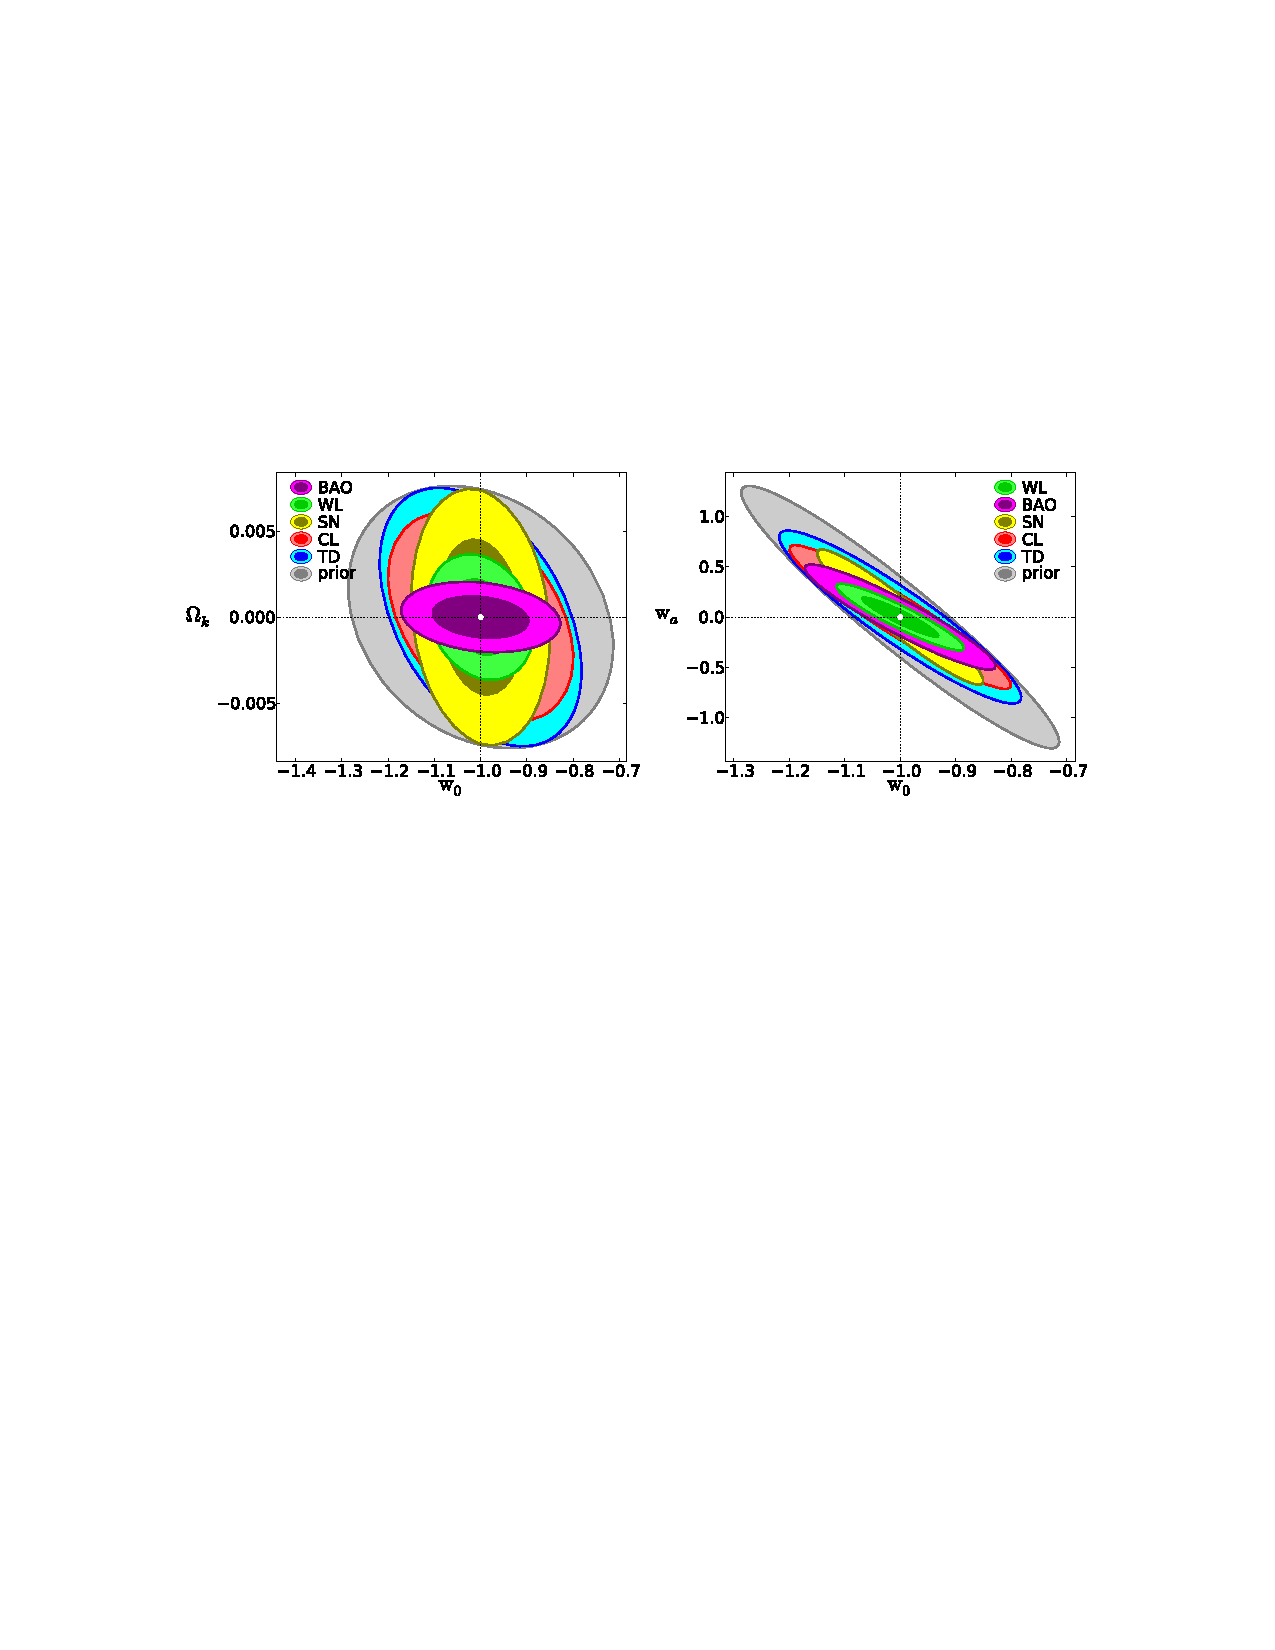
\includegraphics[width=0.9\linewidth]{figs/Coe+Moustakas2009_Figure14.pdf}
    \caption{LSST time delay lens cosmological parameter forecasts (`TD', blue ellipses)
    compared to forecasts from the Dark
    Energy Task Force \citep{DETF} for four other Stage IV probes of cosmology: Baryon Acoustic Oscillations (`BAO'); Weak Lensing (`WL'); Type Ia Supernovae (`SN'); and Cluster counts (`CL').  The parameters considered are the Dark Energy equation of state parameter $w=P/\rho$ evaluated today ($w_0$); its evolution with the scale factor of the Universe in a linear model, i.e. the parameter $w_a$ for the model $w(a) = w_0 + w_a\times(1-a)$; and the curvature of the Universe expressed as a fraction of its critical density, $\Omega_k$.   The prior probability distribution assumed for cosmological parameters is shown in grey.
    A sample of 100 lenses is assumed, each one
    providing a 5\% accurate time delay distance. Figure reproduced from
    \citet{Coe+Moustakas2009}.}
    \label{fig:sl_forecast}
\end{figure*}

% ----------------------------------------------------------------------

\subsection{Technical Description }

% {\it Give a technical description of your program, describing e.g., sample size and properties, justification of spectral or spatial resolution, wavelength, target density, etc.}


%NOAO guidelines:
%The review panel looks to this section to find out about the overall
%strategy of your observational program.  Why do you need the telescopes
%and instruments you request? How are your targets selected?
%Why do you need spectroscopy or imaging, and what measurements will
%you make from the data?  Why is your approach to be preferred over
%some other approach, what must the minimum sample size be to achieve
%your scientific goals (and why), and why are your
%observations likely to be better than previous work in the field?

To be useful as probes of cosmological distances, galaxy scale lenses
need very well constrained mass models. These constraints will come from
two types of targeted follow-up observations:\footnote{
We note that these observations would be taken after targeted optical
spectroscopy to get the redshifts of the deflector and source galaxies.
This can be done at relatively low resolution, but the wider the
wavelength range the better: we will need 3500--10000 Angstroms in the
optical, and maybe a triplespec-like instrument covering the JHK bands
in the IR. Some redshifts may come from overlapping spectroscopic survey
observations, with the systems appearing as composite absorption and
emission line galaxy spectral components. Some of the targeted
spectroscopy could be done at 10-m class facilities.}
\begin{enumerate}
    \item {\bf High Resolution Einstein Rings Imaging} due to the
    source AGN or SN host galaxy. Image quality of $\sim0.1$" or better
    provides the Einstein ring constraints on the lens mass model
    density profile slope (via the arc thickness) that are
    needed to turn each of these systems into a  5\% precision distance
    \citep{MengEtal2015}.
    \item {\bf Spatially-Resolved Spectroscopy of the Lens Galaxy,} enabling
    measurement of the stellar velocity dispersion field to break the
    degeneracy between the predicted time delays and the lens mass
    density profile, calibrating each system to enable it to provide a
    4\% accurate distance.
\end{enumerate}

We now assess the technical  requirements of each of these observations.

{\bf 1. High Resolution Einstein Ring Imaging}:

$\bullet$ Spectral coverage and resolution: imaging in two or three
bands is recommended, to enable clean lens galaxy subtraction.

$\bullet$ Angular resolution: the higher the resolution the better, but
at least $0.1$~arcsec FWMH.

$\bullet$ Depth: the host galaxies of the lensed sources are faint (mag
23--25). Brighter sources will be prioritized when compiling the
follow-up sample, based on analysis of the survey images, and exposure
times of up to 1 hour would be considered, with fainter systems being
discarded \citep{MengEtal2015}.

$\bullet$ Field of view: at least 4~arcsec, to capture the Einstein
ring without dithering.


{\bf 2. Spatially-resolved Spectroscopy of the Lens Galaxy}:

$\bullet$ Spectral coverage and resolution: $R\approx4000-5000$  over a
wavelength range of 1.0--2.2 microns (to cover the Calcium triplet at rest frame
$\sim8500-8700\AA$, or CO at $1.5-1.6\mu$m).

$\bullet$ Angular resolution: 0.1--0.2~arcsec, to resolve the lens galaxy well.

$\bullet$ Depth: the lens galaxies will have brightness in the range
19--22 magnitudes. Again, exposure times of an hour or less will be
considered, with fainter systems being discarded.

$\bullet$ Field of view: at least 4~arcsec, to capture the lens galaxy
within the Einstein ring without dithering.

The above requirements are derived from end-to-end simulations of the
kind carried out by \citet{MengEtal2015}, which will be refined before
proposals to next generation facilities are submitted.

% ----------------------------------------------------------------------

\subsection{Needed Capabilities and Estimate of Demand}

% {\it Describe the needed capabilities and demand (e.g., estimate of observing time) that flow down from the science and technical considerations. If applicable, describe the time critical nature of the required capabilities (do you need to have the capabilities while LSST is carrying out the survey or can you do the follow up later?)}

AO-assisted imaging and integral field spectroscopy on GSMTs would be
best for providing the lens mass model constraints detailed in the
previous section.  We will need capabilities such as those currently
available on Keck, and that will be available on all three of GMT, TMT
and E-ELT (albeit with somewhat different technical specifications).
OSIRIS on Keck is the current best option, even though the field of view
is a bit too small and the current AO system at Keck has relatively low
strehl at 1$\mu$m. The Keck system will be upgraded, but TMT should be
much better: IRIS on TMT would provide the capability we need. Similar
data would be needed for the compound lenses.

The light curves will be accumulated by LSST over the lifetime of the
survey, but we expect accurate cosmography to be possible after the
first 5 years.  Prior to this, the same facilities could be used to good
effect improving the models of lenses found in shallower precursor
surveys such as DES, KIDS and HSC. We expect to have good time delays
for about 30-40 systems before the LSST survey begins: these would be
the targets for high resolution follow-up before 2024, with an
additional 60-70 targets coming from the LSST survey being pursued
between 2024 and 2028 and beyond. The demand is therefore likely to be
around 10-20 systems per year; we assume the higher value below, to help
with planning.

While the targeted observations outlined below would be narrow field,
they would enable a considerable amount of ancillary science, notably in
the areas of dark matter substructure (from perturbations to the imaged
rings) and AGN host galaxy structure.  To summarize, the needs for LSST strong lensing studies are:

{\bf 1. High Resolution Einstein Ring Imaging}:

$\bullet$ Proposed facilities: GSMTs, JWST. 10m-class telescopes for
brighter rings.

$\bullet$ Observations needed: Targeted snapshot (e.g.\ 200--2000
second exposure time with TMT) imaging in the optical and near infra-red.

$\bullet$ Total time required: $\sim30$~hours, depending
on balance between facilities (assuming 20~mins per system, on average),
or $\sim 6$ hours per year.

{\bf 2. Spatially-resolved Spectroscopy of the Lens Galaxy}:

$\bullet$ Proposed facilities: GSMTs, JWST.

$\bullet$ Observations needed: IFU spectra in the near infra-red.

$\bullet$ Total time required: $\sim100$~hours, depending
on balance between facilities (assuming 60~mins per system, on average),
or $\sim 20$ hours per year.

Both the imaging and spectroscopy will be critical for LSST strong lensing cosmology, and hence very important for LSST cosmology considered as a whole.


\section{Science Case 3: Wide Field and Single-Object Spectroscopy for Supernova Cosmology}

\subsection{Science Goals}

Observations of Type Ia supernovae (SNe~Ia) led to the discovery that
the Universe's expansion is currently accelerating
\citep{Riess98:Lambda, Perlmutter99}.  SNe~Ia continue to be a mature
and important cosmological tool \citep[e.g.,][]{Suzuki12, Betoule14,
Rest14}.  Further observations of SNe~Ia will be critical to
improved understanding of the nature of dark energy, perhaps the most
puzzling open problem in all of physics.

LSST will detect and observe $\sim$ $10^{6}$ SNe~Ia out to $z \approx
1$.  With these data, we will be able to measure precise distances and
constrain cosmological parameters.  However, dark energy constraints
are not currently limited by statistics, and even $10^{3}$ SNe~Ia are
more than necessary to reach the current systematic floor
\citep{Betoule14, Scolnic14:ps1}.  While LSST will certainly reduce
some systematic uncertainties (such as those related to calibration),
those related to astrophysics (differences in the SN observables, the
unknown nature of dust, etc) can also be addressed with the proper
auxiliary information.

There are two approaches to using large samples of SNe~Ia for
cosmology.  The first, which has been the standard for more than two
decades, is to use a sample of spectroscopically confirmed SNe~Ia.
The second, which has only just begun to be used for cosmology
\citep{Campbell13}, is to use photometrically classified SNe~Ia.  The
former guarantees that the sample is ``pure,'' consisting of only
genuine SNe~Ia, while the latter is more ``complete,'' but at almost
certainly an equal or lower purity level.  The assumption is that SN
cosmology with LSST will primarily use a photometric sample.

It has been shown that knowing the redshift of a SN significantly
improves its classification and will also reduce distance scatter
some.  Nonetheless, we can make a first pass at classification with
only light curve information (with perhaps including a prior using
photometric redshifts).  The expected path to cosmology will likely
require host-galaxy redshifts.  While a subset of $\sim$ 10\% of the
SNe will be ``hostless'' (having a host galaxy fainter than the
detection limit of the reference image), most host galaxies could be
targeted after the SN has faded.  For the hostless SNe, on the other
hand, we must generally obtain a redshift from the SN itself.  If one
worries about having an unbiased sample, obtaining SN spectra of
hostless SNe would be a priority.

Furthermore, spectroscopy of the SNe themselves provide a test of
photometric classification, improved distance precision
\citep{Bailey09, Blondin11, Foley11:vel}, and additional information
about the explosion.  A subset of SN~Ia spectra will be necessary to
perform the most precise cosmology analysis.

\subsection{Technical Description}

\subsection{Needed Capabilities and Estimate of Demand}

%D) LSS: BAO (including cross-correlation enhancements), redshift-space distortions on cluster or large scales, QSO absorber power spectra \& BAO
% EG, EJ, WD, JN

%E) Science-driven needs for other resources: software, computing and data management resources, access to archival data, etc.
% AB, CS, EG, WD, BW

%\chapter{Science Case 3: Computing, Statistical, and Data Processing Needs}

%\section{Data \& Computing Resources}
\label{sec:datacomp}

{\it Necessary resources for data and computing, beyond core LSST project deliverables, to achieve LSST cosmological science goals. Adam Bolton and others.}

The dark-energy science mission of LSST imposes numerous requirements on 
data resources and computing infrastructure for its success. Many of these requirements 
may be beyond the current baseline for LSST construction 
and operations, and some may also be beyond capabilities currently 
anticipated within the DOE-supported LSST Dark-Energy Science Collaboration (DESC)\@.
This section describes these required capabilities as they flow from dark-energy 
science requirements.

\subsection{Data-set access and definition}

The analysis of large LSST datasets for derivation of dark-energy parameter constraints 
will involve development and application of analysis codes by large teams of 
scientists working over periods which are likely to extend over many years, and which will 
require long-term stability and accessibility for scientific reproducibility. This translates 
into requirements that LSST's released static-sky datasets be: 

\begin{itemize}
\item Version controlled
\item Exposed through machine-readable programmatic interfaces
\item Maintained on accessible storage resources for many-year timescales
\end{itemize}

\subsection{Combination of LSST data with other data sets}

Multiple dark-energy science analyses of LSST data will rely on the combination 
of LSST data with redshifts and object parameters from other surveys (both imaging 
and spectroscopic). These analyses impose requirements for: 

\begin{itemize}
\item Long-term access to curated copies of auxiliary datasets
\item Computing infrastructure sufficient for co-analysis of LSST data with auxiliary data
\end{itemize}

\subsection{Likelihood characterization}

Cosmological analyses of LSST data sets will require accurate physical characterization of 
the populations of tracer objects used. This will be necessary both to understand the 
selection-functions of the samples themselves and their evolution with redshift, 
and to connect with physical models for the bias recipes through which these 
populations are related to the underlying dark-matter distribution. In many instances, the 
salient physical parameters of tracers in LSST data may be measured at a level of significance 
that does not admit sufficient characterization through simple Gaussian errors or covariances. 
Such analyses will therefore require: 

\begin{itemize}
\item Explicit identification of all LSST catalog-object 
parameters that are relevant as input to cosmological analysis
\item Sufficient characterization of the joint likelihood of these measured 
parameters on an object-by-object basis, either through direct reporting 
within LSST catalogs, or through custom determination using LSST Level 3 
software infrastructure
\end{itemize}

\subsection{Redshift data validation}

Cosmological analyses of LSST data that rely on spectroscopic redshifts will impose requirements on 
the quality of those redshift data in terms of completeness, purity, precision, and accuracy. In the case 
of spectroscopic samples adopted from other surveys, the requirements for LSST analysis may be 
different than those imposed by the primary science case of those other surveys. Therefore, all 
spectroscopic samples used in LSST dark-energy science analysis will require: 

\begin{itemize}
\item Quantitative specification of the science requirements for redshift and parameter measurements
\item Controlled software infrastructure for validating spectroscopic catalogs 
against LSST dark-energy science requirements
\item Software-development infrastructure for the modification of redshift- and parameter-measurement codes, 
for cases in which a failure to meet requirements is traced not to spectroscopic target-selection or 
observing, but rather to the analysis software used for delivering redshifts from the data
\end{itemize}

\subsection{Mock catalogs}

Simulations, and mock catalogs based on those simulations, will be necessary for multiple 
dark-energy science applications of LSST. These include the characterization of covariances in 
large-scale structure measurements across length scales, determination of the statistics of 
line-of-sight density projection effects for strong-lensing systems, and forward modeling 
of statistical estimators as a function of cosmological parameters. These applications will require: 

\begin{itemize}
\item Allocation of sufficient computing and storage resources to conduct suites of cosmological 
$N$-body simulations tailored to LSST dark-energy science analysis
\item Support for the generation, documentation, and application of mock LSST catalogs based on 
appropriate simulations.
\end{itemize}

\subsection{Survey characterization}

Precision cosmological measurements of the baryon acoustic oscillation (BAO) feature using LSST
data will be sensitive to percent-level systematics that may vary across the LSST footprint in a 
complex field-dependent geometric pattern. In order that these variations do not compromise 
the precision and accuracy of the cosmological measurements, the following capabilities 
will be required: 

\begin{itemize}
\item Sufficient analysis within core LSST observing and data-reduction operations to enable 
determination of field-dependent quantities relevant for dark-energy science analysis 
\item Computation of weight-masks for bright stars, stellar number density, effective seeing, and 
effective depth in LSST static-sky data releases, along with a documented and 
supported data-model for the encoding of these masks
\item Software infrastructure for incorporating these masks into LSST dark-energy parameter analysis
\end{itemize}




%F) Development of statistical techniques; e.g. for utilizing photo-z pdf information/samples for, e.g. clustering measurements.  Developing techniques for probabilistic inference over redshift distributions
% CS, EG, JN, WD, BW, EJ

%
LSST will generate very large galaxy samples that can be used for
investigations of the galaxy distribution -- e.g. correlation
functions, luminosity functions, dependence on environment -- that are
much more sensitive than what we are used to. These will enable
measurement of features and evolution at high precision. At the same
time, these samples will largely rely on photometric redshifts. To
take full advantage, and to avoid introducing subtle systematics,
astronomers will have to develop methods that use the full information
in the photo-z P(z) estimate, rather than using point estimates
(placing galaxies at their best estimate redshift).

This will require developing techniques for probabilistic inference
over photo-z probability distributions, when measuring typical
population estimates such as the luminosity function or correlation
function. It will generally not be practical to forward-model the
entire dataset (e.g. constraining the luminosity function directly
from galaxy apparent magnitudes, in principle would require modeling
the LF and colors of all galaxies at all redshifts). So investigators
will use photo-z probability distributions calculated either by the
LSST pipeline or their own.  Generalizing the standard measurements to
use the information in the P(z) distribution and to be robust against
errors in estimating P(z) is a relatively unexplored area. Simple
ideas such as randomly sampling from each galaxy's P(z) can give wrong
answers (because this magnifies photo-z spread rather than
compensating for it). Exploiting the LSST dataset will require
supporting research into methods for inference using photo-zs and
supporting the community in developing and releasing publicly
available code and tools.


%\section{Dark matter in galaxy clusters}

%Cosmology with the cluster mass function may become one of the most powerful probes of the cosmology in the LSST era, if cluster masses can be measured to high enough accuracy and precision (Cosmic Visions report; Krause and Eifler 2016).  Moreover, they provide avenues for probing gravity as well as the properties of dark matter.  Multi-object spectroscopy plays a major role on all of these:

\begin{itemize}
\item Photo-z uncertainties specific to cluster fields present one of the primary systematics in cluster weak-lensing analyses to anchor the absolute cluster mass calibration (Applegate et al. 2014, DESC white paper).  Galaxies along a line of sight that contains a cluster are more likely to be at the cluster redshift than would be expected based upon posterior probability distributions calculated without any reference to position.  Such modulation of the prior should depend upon both cluster redshift and mass.  Some amount of training datasets (targeting galaxies selected by their photo-z's to be behind clusters) is necessary for this work to identify (possibly unexpected) failure modes of mistaking cluster galaxies for background galaxies. FOVs of $\gtrsim 20$~arcmin are ideal for targeting cluster fields at $z_{\rm Cl}\gtrsim0.2$.  Constraints on the wavelength coverage are somewhat reduced for investigating only the cluster redshift failure mode. Accordingly, existing instruments (e.g. DEIMOS) are already well-suited for this work, especially if the large-scale photo-z training surveys are predominantly performed with larger-area, sparser spectrographs.  Training sets should target clusters over a range of redshift, acquiring ~500 background redshifts per cluster to fully characterize the accuracy of $p(z)$ distributions in cluster fields.  In addition, cross-calibration datasets can be a sensitive test for residual cluster galaxy contamination. These are easier to obtain, targeting (bright) red-sequence galaxies.  Spectroscopy of $\sim 100--300$ galaxies in each of $\sim 20--50$ clusters would be useful for this purpose.  
\item The combination of weak lensing with dynamical mass probes (e.g., measurements of galaxy velocities within clusters) can be used to test non-GR theories of gravity, which could provide an alternative explanation for the cosmic acceleration commonly described to dark energy. The same spectroscopy used to characterize photometric redshifts around clusters can be used to measure infall velocities and hence provide constraints on the origin of cosmic acceleration, if the FOVs extend to $\gtrsim 2h^{-1}$ Mpc from the cluster centers.
\item As the most massive collapsed structures in the Universe, the structure and evolution of clusters is sensitive to the properties of dark matter, although is it challenging to separate non-standard-DM signatures from the effects of baryonic physics (Peter et al. 2013). In merging clusters, the effects e.g. of self-interacting dark matter may be most apparent.  LSST (with eROSITA) will identify hundreds to thousands of (major) mergers, but kinematic information is critical to reconstruct the merger histories and geometries. Instruments with $\sim 15-20$~arcmin FOVs and high-multiplexing capabilities are again well matched. {\bf Ask Will to write, and check with Annika.  Should also include bulleticity?}
\end{itemize}

%\subsection{Science Goals}
%
%Describe your science goals here, as in the scientific justification of an NOAO proposal. If you have multiple science goals, you can either describe them all here, or replicate the science, technical, and capabilities sections for each goal. Just create one summary table for the entire program.  
%
%%NOAO guidelines:
%%
%%The scientific justification should explain the overall goals of
%%your program in the context of your field, as well as the importance
%%of your program to astronomy.
%%Writing a good scientific justification is an art.  It takes
%%skill and practice.  And it requires a good scientific idea.
%%This last you must supply but a few general guidelines
%%about proposal writing might still be helpful...
%%
%%\begin{itemize}
%%\item
%%State succinctly and clearly the problem you are trying to solve
%%and the progress that will be made toward doing so if the proposed
%%observations are successful.  If the review panel members have to work hard
%%even to understand what you want to do, they are unlikely to be
%%sympathetic to your proposal.
%%
%%\item
%%Explain clearly why the project is important and how it
%%relates to the broad context and important issues in your field.
%%Many proposals focus too tightly on a specific observational
%%goal (e.g. ``measure the velocity dispersion of this cluster of galaxies'')
%%without explaining why it is important or how it relates to a
%%significant question about the Universe.
%%
%%\item
%%Be specific.  If your observations will ``constrain theoretical
%%models,'' then discuss what will be constrained and why those
%%constraints matter.  Make sure the review panel understands exactly why
%%the observations you propose will make a difference in your field,
%%and exactly how the observations will refine or
%%require changes in the theory.
%%
%%\item
%%Keep it simple.  Try to focus on the central idea of your proposal.
%%Complex arguments are hard to explain and hard for the panel members to follow.
%%Distracting tangential arguments obscure the theme of your proposal.
%%
%%\item
%%Include a figure to help explain what you want to do.  Sample
%%data or model predictions shown in a figure often help clarify
%%complex arguments for the panel members.
%%
%%\item
%%Keep it short.  Never exceed a page for the text of the scientific
%%justification, and never reduce the font size.  It may even help to
%%be a little under a page, and increase the font size a little!
%%Organize your presentation with paragraphs, headings, and bullets
%%so it is easy to read.
%
%
%
%\subsection{Technical Description }
%
%Give a technical description of your program, describing e.g., sample size and properties, justification of spectral or spatial resolution, wavelength, target density, etc.
%
%
%%NOAO guidelines:
%%The review panel looks to this section to find out about the overall
%%strategy of your observational program.  Why do you need the telescopes
%%and instruments you request? How are your targets selected?
%%Why do you need spectroscopy or imaging, and what measurements will
%%you make from the data?  Why is your approach to be preferred over
%%some other approach, what must the minimum sample size be to achieve
%%your scientific goals (and why), and why are your
%%observations likely to be better than previous work in the field?
%
%
%
%\subsection{Needed Capabilities and Estimate of Demand}
%
%Describe the needed capabilities and demand (e.g., estimate of observing time) that flow down from the science and technical considerations. If applicable, describe the time critical nature of the required capabilities (do you need to have the capabilities while LSST is carrying out the survey or can you do the follow up later?) 



%\bibliographystyle{fapj}
\bibliography{dark_energy}{}
\bibliographystyle{apj}

\end{document}
